\begin{figure}[h!]
	\centering
	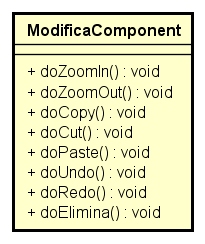
\includegraphics[scale=0.8]{res/sections/SpecificaFrontEnd/Components/Disegnetti/modifica.png}
	\caption{Diagramma della classe ModificaComponent}
\end{figure}

\begin{itemize}
	\item \textbf{Descrizione:}\\
	È il componente che descrive la voce \textit{Modifica} del menu dell'editor.
	\item \textbf{Utilizzo:}\\
	
	\item \textbf{Metodi:}
		\begin{itemize}
			\item \emph{+doZoomIn()}\\
    		Esegue lo zoon in avanti
    		\item \emph{+doZoomOut()}\\
    		Esegue lo zoom in indietro
    		\item \emph{+doCopy()}\\
    		Esegue il comando copia del menu
    		\item \emph{+doCut()}\\
    		Esegue il comando taglia del menu
    		\item \emph{+doPaste()}\\
    		Esegue il comando incolla del menu
    		\item \emph{+doUndo()}\\
    		Annulla l'ultima azione compiuta
    		\item \emph{+doRedo()}\\
    		Ripristina l'ultima azione annullata
    		\item \emph{+doElimina()}\\
    		Elimina l'elemento selezionato nell'editor	    		
		\end{itemize}
\end{itemize}